\chapter{Documentation}
J'allais commencer la création des messages quand mon maître d'apprentissage m'a demandé de réaliser une documentation sur les messages de BL, afin que personne n'ait à refaire le travail que j'ai eu à mener au début du projet.

~

Au fur et à mesure que je travaillais sur l'écriture du message (détaillée au chapitre \ref{creation_message}), j'ai rédigé un rapport sur l'ensemble des segments que l'on peut rencontrer dans un document de BL. J'ai essayé de faire un document tel que j'aurais voulu avoir pour me guider.

Afin de faire les choses complètement, je l'ai découpé en deux parties.


\section{Données et conditions}
Comme je l'ai dit précédemment, les données nécessaires à la création d'un document BL sont nombreuses. Mais ce sont surtout les conditions portant sur ces données qui sont importantes. Dans quel cas telle ou telle valeur est-elle obligatoire ? Quand mon port de destination est le Canada, quelles sont les données qui deviennent obligatoires ?

~

C'est en cherchant à répondre à ces deux questions que j'ai construit cette première partie de la documentation. Pour chaque donnée, j'indique les champs qui la rendent obligatoire ou optionnelle, ainsi que les données qui dépendent de sa présence / absence.


\section{Contenu des segments}
La seconde partie est la plus longue, mais je pense que c'est aussi la plus utile. Elle commence par une sorte de sommaire, qui récapitule le nom de chaque segment pouvant être présent. Il permet aussi de connaître l'ordre dans lequel sont sensés s'écrire les segments (un document commence systématiquement par un UNH, suivit d'un UNB, etc.)

~

Chaque segment est présenté de la même manière. Ce qui suit est la présentation typique d'un segment mais certains, notamment ceux dont le format change en fonction d'autres variables, peuvent présenter des différences.

Voici donc un exemple de segment :
\begin{figure}[!ht]
	\begin{center}
		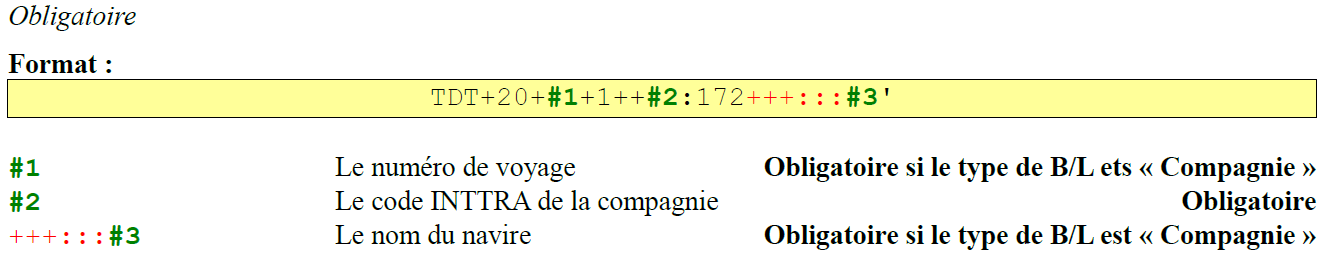
\includegraphics[scale=.53]{Contenu/ProjetTuteure/Images/Segment_TDT.png}
	\end{center}

	\caption{Détails du segment \og TDT \fg}
\end{figure}

Détaillons maintenant son contenu. Sur la toute première ligne (en italique), est indiqué si le segment est obligatoire ou non, avec de possibles indications supplémentaires. Exemple : \og Non obligatoire, sauf si le port de destination est le Brésil \fg.

~

Vient ensuite un aperçu de segment lui-même, ces variables étant remplacées par des dièses numérotés. Certains séparateurs (\textbf{+} ou \textbf{:}) peuvent apparaître en rouge. Cela signifie que leur présence est liée à la variable qui les précède ou les suit. Par exemple, dans notre cas, les \og +++::: \fg{} qui précèdent \#3 ne sont à insérer que si celui-ci est présent.

~

Puis chaque variable est détaillée. A gauche, le numéro de la variable est affiché précédé ou suivit par les séparateurs qui lui sont attribués. Au centre, il y a une brève description du contenu de cette variable. Pour finir, sur la droite, j'indique si la variable est obligatoire ou non. Par exemple, dans notre cas, le nom du bateau est obligatoire si le message est adressé à une compagnie maritime, mais peut être omis dans le cas d'une NVOCC.

Chaque ligne détaillant une variable peut également être suivie d'une seconde ligne en italique, qui donne des précisions sur le contenu de la variable, comme la liste des valeurs autorisées ou encore le format (exemple : code postal concaténé au nom de la ville).